\chapter{Introducción}
Este proyecto es software libre, y está publicado con la licencia \cite{gplv3} General Public License v3.
Se puede acceder a través de GitHub en este \href{https://github.com/pablojjimenez/TFG}{enlace} puedes sentirte libre de contribuir mediante una solicitud de fusión o \textit{Pull Request}. También forma parte de los \href{https://github.com/JJ/TF-libres-UGR}{trabajos liberados}\footnote{https://github.com/JJ/TF-libres-UGR} de la UGR.

\section{Motivación} 
El tratamiento automático de la información por medio de técnicas matemáticas procesadas por un ordenador ha cambiado la forma en la que nos organizamos, estudiamos y obtenemos conclusiones.

Siempre he creído que la evolución en nuestra calidad de vida pasa por un
conjunto de soluciones informáticas que han de colaborar entre ellas para obtener tal propósito. 
En esta última década la recolección y almacenamiento de datos es una actividad transversal incesante que sin un tratamiento científico no nos aporta valor. 

Los servicios sanitarios suponen un eje vertebrador cuando hablamos de mejorar la calidad de vida de las personas. Numerosos estudios sociológicos avalan que la sanidad es una preocupación incesante de los españoles, más aún si cabo tras la pandemia que hemos atravesado. 

\begin{figure}[]
	\centering	
	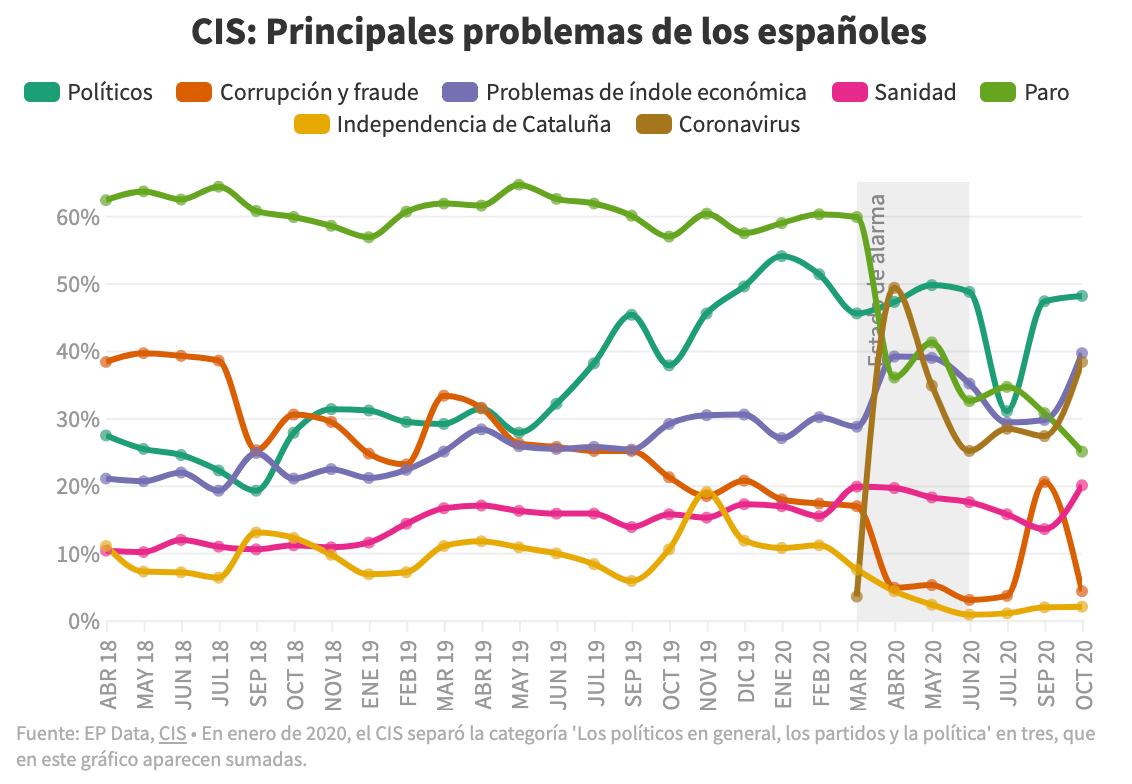
\includegraphics[scale=0.5]{doc/logos/imgs/CIS_1.png}
	\caption{ Principales problemas de los españoles según el CIS. \hyperref[Enlace al artículo]{https://www.rtve.es/noticias/20201015/crisis-economica-coronavirus-preocupan-ahora-mas-espanoles-paro/2045610.shtml} }
    \label{fig:worst_f_value}
\end{figure}

Como podemos observar en la gráfica superior; En la preocupación de los españoles la sanidad siempre se muestra con una tendencia al alta a pesar de no estar exenta de movimientos sinusoidales. Esta tendencia solo es superada por el paro y problemas relacionados de índole económico.

La transparencia mantiene a la población tranquila y a pesar de que estos datos sean accesibles para la población sin un tratamiento informático y matemático de estos es como si no estuvieran. Mi tarea es facilitar los estudios sobre la evolución de las defunciones según causa de muerte aprovechando los datos públicos que se publican anualmente.

Ahora mismo es imposible poder consultarlos para obtener información concreta y útil. No podemos consultar estos datos por variables, muy lejos estamos de poder realizar visualizaciones o tener aplicaciones que sean capaces de obtener valor a partir de estos datos.

\section{Usuarios}
\label{sec:usu}
Una de las herramientas que nos permiten definir el alcance y las necesidades de la aplicación es la creación de perfiles de personas ficticias, candidatos diana a utilizar el sistema en un futuro.

De esta forma, podemos justificar las decisiones tomadas en aras de alcanzar el objetivo por parte de los usuarios interesados en el producto final. La función de estos usuarios es poder crear posteriormente historias de usuario que identifiquen los problemas y deseos de los usuarios para que posteriormente en equipo de desarrollo pueda proponer una solución.

He creado dos someras personalidades lo más variopintas posibles en aras
de enfocarnos más aún en el usuario y dotar de mayor calidad el resultado final, de modo que podamos abarcar por completo las necesidades de estos.

\rowcolors{1}{gray!20}{gray!8}
\begin{table}[H]
	\begin{center}
		\begin{tabular}{| p{\dimexpr 0.25\linewidth-2\tabcolsep} |
                   p{\dimexpr 0.8\linewidth-2\tabcolsep} |}
			\hline
			Persona 1 &  \\ \hline
			\textbf{Nombre} & Raquel \\
			\textbf{Edad} & 30 años \\
			\textbf{Formación} & Senior frontend developer \\
			\textbf{Personalidad} & \begin{itemize}
                \item Deportista.
                \item Tímida.
                \item Lógica.
            \end{itemize} \\
			\textbf{¿Cuál es su entorno?} & \begin{itemize}
                \item Sus amigos.
                \item Su gato.
                \item Sus libros.
            \end{itemize} \\
			\textbf{¿Qué dispositivos utiliza en su día a día?} & \begin{itemize}
                \item Un portátil.
                \item Un smartphone.
            \end{itemize} \\
            \textbf{¿Cuál es su actitud hacía la tecnología?} & \begin{itemize}
                \item Perezosa.
                \item Sabe programar.
            \end{itemize} \\
            \hline
		\end{tabular}
		\caption{Usuario ficticio 2}
	\end{center}
\end{table}

\rowcolors{1}{gray!20}{gray!8}
\begin{table}[H]
	\begin{center}
		\begin{tabular}{| p{\dimexpr 0.25\linewidth-2\tabcolsep} |
                   p{\dimexpr 0.8\linewidth-2\tabcolsep} |}
			\hline
			Persona 3 &  \\ \hline
			\textbf{Nombre} & Isabel \\
			\textbf{Edad} & 45 años \\
			\textbf{Formación} & Matemática \\
			\textbf{Personalidad} & \begin{itemize}
                \item Aventurada.
                \item Protagonista.
            \end{itemize} \\
			\textbf{¿Cuál es su entorno?} & \begin{itemize}
                \item Su familia.
                \item Sus padres.
                \item Su trabajo. Profesora en la UGR.
            \end{itemize} \\
			\textbf{¿Qué dispositivos utiliza en su día a día?} & \begin{itemize}
                \item Un ordenador de sobremesa.
                \item Un smartphone.
                \item Un iPad que comparte con su marido.
            \end{itemize} \\
            \textbf{¿Cuál es su actitud hacía la tecnología?} & \begin{itemize}
                \item Valiente.
                \item Proactiva.
            \end{itemize} \\
            \hline
		\end{tabular}
		\caption{Usuario ficticio 3}
	\end{center}
\end{table}


\section{Objetivos}
\label{sec:obj}
El objetivo principal de este proyecto es que el sistema sea capaz de darle a los usuarios la capacidad de conocer la evolución de las causas de muerte. De forma que se pueda consultar de forma sencilla los datos almacenados. Las causas de muerte están clasificadas según la Clasificación Internacional de Enfermedades y se encuentran clasificadas en base a distintas variables. El sistema debe de atender a los usuarios diana de la app que como he comentado en el apartado anterior, para identificarlos se ha utilizado la herramienta de personas ficticias. 
